\documentclass{beamer}
\usepackage{graphicx}
\usepackage{listings}
\usepackage{beamerthemesplit}
\usetheme{Warsaw}

\title{Moogle!, ligth fast searching}
\author{Víctor Vena}
\date{16 de julio de 2023}



\begin{document}

\begin{titlepage}
   \begin{center}
    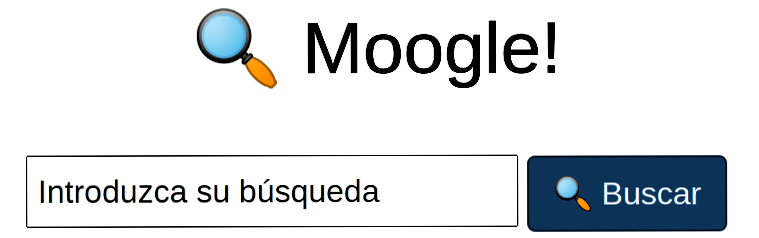
\includegraphics[scale=0.25]{Imagenes/moogle.png}
   \end{center}
\end{titlepage}

\centering

\section{Qué es Moogle!}
Moogle! es un motor de búsqueda con una interfaz amigable basada en web y búsquedas ligth fast.
\pagebreak

\section{Caracteristicas}
\begin{itemize}
    \item Búsquedas rápidas. Ofreciendo resultados al momento.
    \item Búsquedas inteligentes
    \begin{itemize}
        \item Determina los términos más relevantes y prioriza los documentos que los contienen
        \item Muestra los resultados más importantes primero
    \end{itemize}
    \item Muestra fragmentos de los documentos.
    \item Ofrece alternativas ante palabras mal escritas o que dan pocos resultados.
\end{itemize}
\pagebreak

\section{Proximamente}
Posibilidad de configurar Moogle! para que realice las busquedas en cualquier directorio que se desee.\\

\pagebreak

\section{Despedida}
Esto es todo, espero disfruten Moogle!

\pagebreak

\maketitle

\end{document}